\documentclass[a4paper, 12pt]{article}
\usepackage{listings} 
\usepackage{xcolor}
\usepackage{mdframed}
\usepackage{graphicx}
\usepackage{pgfplots}

% Allows for floating images
\usepackage{float}
\usepackage{mathtools}

% Custom 1 inch margins
\usepackage[margin=1.00in]{geometry}

% Custom Floor and Ceiling operators
\DeclarePairedDelimiter\ceil{\lceil}{\rceil}
\DeclarePairedDelimiter\floor{\lfloor}{\rfloor}

% Custom background color for code listings
\definecolor{code-gray}{gray}{0.93}

% Beginning of document
\begin{document}
\title{ECE 443 - Homework \#2}
\author{Collin Heist}
\date{\today}
\maketitle
\pagenumbering{arabic}

\section{Findings}
Observing the behavior of \textbf{LEDA} and \textbf{LEDB} shows that the kernel switches what task is \emph{running} at a one millisecond interval. This is obvious because the 'on' LED alternates between A and B every millisecond -- which is shown in Figure~\ref{fig:img00}.

One facet of the task execution behavior that is not very well illustrated in this lab is how each task is technically being run \emph{constantly} during the entirety of its corresponding one millisecond period. Just looking at Figure~\ref{fig:img00}, it might be believed that each task executes just \emph{once} before going idle and switching over to the next task at the next increment of a millisecond. However, what's actually happening here is that the task is rerunning constantly, except the \textbf{if} statement only evaluates to \textbf{true} on the first run, because afterwards the LED is on, and the statement is \textbf{false}.

\section{Results}
Below is the waveform captured using the \textbf{Waveforms} program. DIO 1 is \textbf{LEDA} and DIO 0 is \textbf{LEDB}. What should be clearly seen is that the 'active' LED alternates each millisecond.

\begin{figure}[H]
\centering

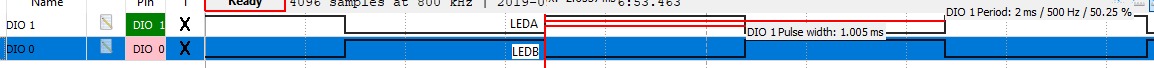
\includegraphics[width=\textwidth]{img00.png}
\caption{Behavior of \textbf{LEDA} and \textbf{LEDB} in the project}
\label{fig:img00}
\end{figure}

\end{document}